
\chapter{Mobile Web (e App)}
	Solo recentemente i dispositivi mobile hanno spopolato è la tecnologia ha superato di gran lunga i web designer che sono impreparati nell'ambito mobile emergente. Nel 2013 l'accesso a internet da dispositivi mobile ha superato quello di desktop e laptop ed è in costante crescita. Nonostante questo trend, 530 siti nella top 1000 del mondo non dispongono di una versione mobile e il 25\% di questi sfora lo schermo.

	\section{Un po' di storia}
		Nel marzo 2013 avviene un importate scelta aziendale in Google. Il team di sviluppo di Android che non portava risultati soddisfacenti è inglobato dal team di Chrome che invece aveva successo. L'idea era ed è quella di avere convergenza tra mondo mobile e web. 
		
		Già prima si era cercato di percorrere questa rotta da Google ma le cose non andarono bene visti i contrasti con Apple che non voleva collaborare. Si pensi che lo stesso Steve Jobs era contrario alle app. Da qui il motivo dell'acquisto del sistema Android da parte di Google.
		
		Ora il percorso è ben delineato: la nascita delle hybrid apps scritte usando HTML5 e multipiattaforma segnano ancora più visivamente la convergenza tra mobile e web.
	
	\section{Le App}
		Nascono dalla necessità di minimizzare ancora una volta lo sforzo computazionale delle persone. L'app minimizza enormemente il tempo di accesso al servizio richiesto dagli utenti. Di conseguenza questo porta a maggiori esigenze da parte degli utenti e riduce i timer di soddisfazioni.
		
		\subsection{Parlano le statistiche}
			Dalle statistiche emerge:
			\begin{itemize}
				\item quasi un quarto degli utenti usano app più di 60 volte al giorno 
				\item e questo cresce ogni anno del 123\%!
				\item La fascia d'età che meno 'drogata' di app si trova tra i 25 e 35 anni (i motivi sembrano principalemente per la mancanza di tempo).
			\end{itemize}

			Le app vincono sul mobile web, gli utenti smartphone passano in media l'84\% di tempo giornaliero sulle app e solo il 14\% sul web vero e proprio. Nella pratica si capisce il perché:
			\begin{itemize}
				\item il 32\% di questo tempo è speso in \textbf{giochi} (non sorprende quindi la scelta del nome Google Play per lo store di Google).
				\item il 28\% sui \textbf{social}, il 17\% è Facebook!
			\end{itemize}
			Da notare che tutto questo uso di app (giochi a parte) è solo fruizione di contenuti nel web tramite l'app apposita.
			
		\subsection{L'arena delle App}
			Quando le statistiche parlano chiaro e muovono un sacco di persone si muovono anche un sacco di soldi e ricerca di successo. È per questo motivo che nel mercato delle app, attualmente, c'è un'enorme competizione:
			\begin{itemize}
				\item Le app hanno vita media bassissima: dai \textbf{4 mesi} ad \textbf{1 anno}.
					\begin{itemize}
						\item i game hanno vita media di soli \textbf{4 mesi}.
					\end{itemize}
				\item Se un app resiste ed è ancora in crescita dopo 3 mesi avrà una vita lunga altrimenti è defunta e da considerarsi un insuccesso.
			\end{itemize}
			
			\subsection{La sequenza della morte}
				Di seguito quella che viene chiamata la \emph{sequenza della morte} di una app descrive al meglio quello già descritto sopra, riportano i dati del comportamento degli utenti di fronte ad un'app.
				\begin{itemize}
					\item il \textbf{26\%} delle app è aperta al massimo \textbf{una volta}.
					\item il \textbf{13\%} sono aperte al massimo \textbf{2 volte}.
					\item il \textbf{9\%} sono aperte al massimo \textbf{3 volte}.
					\item il \textbf{50\%} degli utenti apre le app al massimo 3 volte e poi basta.
				\end{itemize}
		
		\subsection{Alla ricerca dell'App}
			Tanta competizione e tante app defunte in pochissimo tempo. Ma come trovare queste app? È qui che il paragone con i siti web è possibile. Come per essi esistono i motori di ricerca anche per le app esistono questi: gli store. Anche qui infatti si presenta il problema di essere trovati ai primi posti della ricerca nello store proprio come per i siti internet. Per fare ciò è nata l'ASO.
			
			\subsection{ASO: App search optimization}
				È il corrispondente CEO per le app e presenta di fatto delle somiglianze prima su tutte funziona per \emph{keywords} che richiede quindi sforzo per un'\textbf{ottimizzazione testuale} sui pochi luoghi disponibili nello store.
				\begin{itemize}
					\item Descrizione app.
					\item Spazio apposito per le keyword.
					\item Nome dell'app (corrisponde al nome del sito vedere indice NOMI).
				\end{itemize}
				Poichè non si possono utilizzare tecniche ipertestuali i motori di ricerca degli store applicano l'uso dei dati del sistema sociale complessivo (SIS) che si basa su quanto segue:
				\begin{itemize}
					\item numero di download (integrati nel tempo).
					\item tempo d'uso dell'app.
					\item \emph{ratings} e \emph{review}.
					\item disinstallazioni.
					\item brand.
					\item metriche di motori di ricerca del web. Per esempio su Google Play sono integrate tutte le metriche positive e negative raccolte sul web per quell'app.
				\end{itemize}
							
			
	\section{Usabilità: mobile e desktop}
		Per valutare se una pagina è corretta per dispositivi mobile esistono potenti strumenti. Prima fra tutti il \emph{Google mobile compatibility test}. Esso verifica che siano rispettate alcune caratteristiche che possiamo catalogare in tre componenti base:
		\begin{enumerate}
			\item Essere mobile.
			\item Taglia dello schermo.
			\item Interazione.
		\end{enumerate}
		
		\subsection{L'esempio di Facebook}
			Una considerazione è doverosa farla sui diversi tipi di device oggi in commercio. Oltre a diverse composizioni hardware abbiamo diverse funzionalità offerte dagli telefoni cellulari. Bisogna porre attenzione al target di riferimento, si pensi ad esempio che non tutti i telofoni hanno il touch.
			L'esempio del social network mondiale Facebook è esplicativo del problema. Facebook per risolvere questi problemi infatti offre addirittura 3 versioni mobile del sito \emph{facebook.com}:
			\begin{description}
				\item [m.facebook:] versione per cellulari non touch.
				\item [touch.facebook:] versione per cellulari touch.
				\item [0.facebook:] versione a banda ultra ridotta offerto gratuitamente in tutte le zone dove le reti telefoniche sono lente (fidelizzazione globale dei clienti).		
			\end{description}
		
		\subsection{Essere Mobile}
			Essere mobile significa avere un diverso collegamento alla rete: la rete mobile con tutte le conseguenze ovvie.
			Le connessioni 3G in media sono il 40\% più lente delle normali connessioni questo significa che ogni sito web mobile sarà caricato con il 40\% in più di tempo. Un disastro se pensiamo ai già discussi timer dell'utente. Fortunatamente con le nuove tecnologie per la rete mobile, il 4G/LTE abbiamo reti in media il 12\% più lente.
			
			\subsubsection{Timer su mobile}
				Abbiamo visto che i timer causa connessioni di rete mobili si sono allungati del 40\%, ma cosa ancora peggiore ad ogni pagina/click l'utente accumulerà un ritardo del 40\%. Per far fronte a questo problema e ridurre un po' i timer bisogna ridurre il più possibile il carico delle pagine (0.facebook.com). 
				\begin{itemize}
					\item Nel caso \textbf{desktop} l'utente aspetta \textbf{al massimo 2 secondi} prima che inizini le brutte sensazioni.
					\item Nel caso \textbf{mobile} abbiamo la stessa identica cosa!
				\end{itemize}
				\begin{quote}
					\emph{``Non basta cambiare il layout per supportare il mobile."}  
				\end{quote}
			\paragraph{Responsivenes}
				Lo stesso discorso vale anche per le app, l'azione richiesta dall'utente non deve metterci più di 2 secondi. Si deve seguire il principio della \emph{responsivenes}: non si deve mai far percepire il ritardo agli utenti se non in casi speciali segnalati all'utente.
				
			\subsubsection{Alla ricerca di soluzioni}
				\begin{description}
					\item[Progress bar e spinner:] visto questo inghippo potremmo usare qualcosa per allietare il ritardo inevitabile attraverso tecniche già usate dal lato desktop come \emph{progress bar} e \emph{Spinner}. NO! In qualsiasi caso, anche su desktop, tecniche del genere sono risultate spiacevoli per l'utente. L'effetto è come quello di essere in coda e avere una voce che costantemente ti ricorda di esserlo.
					\item[Transitionig:] tecnica più apprezzata rispetto le precedenti che si propone di tenere impegnato l'utente con un'animazione. Un esempio possiamo trovarlo dal vecchio Netscape che adoperava questa tecnica nel caricamento delle pagine (\emph{skleton screen}). Esse infatti venivano generate e mostrate man mano che venivano scaricati i dati completamente.
					\item[Preemptiveness:] tecnica che consiste nel far fare qualcosa preventivamente all'utente. Si prenda per esempio l'upload di foto di \emph{Whats App}, l'utente è intrattenuto da una schermata dove viene richiesto un commento testuale prima di inviare il messaggio. In realtà l'app sta utilizzando quel tempo per caricare la foto. Foto caricata, nessuna apparente attesa, utente contento.
				\end{description}
				
		\subsection{Taglia dello schermo}
			Un'altra caratteristica fondamentale del mobile che impatta enormemente sull'usabilità è la taglia dello schermo. Una pagina classica farà fatica ad evitare lo scroll. Abbiamo visto gli effetti dello scroll su desktop, ma su mobile?
			\begin{itemize}
				\item Lo \textbf{scroll orizzontale} resta il \textbf{male del male}.
				\item Lo \textbf{scroll verticale} non è così male come lato desktop.
			\end{itemize}
			
			\subsubsection{Scroll verticale su mobile}
				\begin{itemize}
					\item lo sforzo fisico e mentale è minimo a differenza del desktop.
					\item ma risulta deleterio per mostrare scelte quali possono essere liste di prodotti, perché richiede uno sforzo di memoria.
				\end{itemize}
				Per guadagnare un po' di spazio e ridurre lo scroll:
				\begin{itemize}
					\item Nelle scelte si evita del tutto l'uso di immagini, restringerle non è cosa gradita.
					\item Utilizzare le icone al posto del testo, attenzione però a rispettare:
					\begin{description}
						\item [explainability:] fornire informazioni testuali se si posiziona il cursore.
						\item [escapability:] possibilità di evitare l'azione se ho già premuto ma non rilasciato. 
					\end{description}
				\end{itemize}	
				
				Una nota per l'uso delle icone. Si ricorda che gli utenti preferiscono \textbf{sempre} il testo (vedi confronto tra web e giornali). Si pensi che per abituare gli utenti all'uso dell'icona hamburger, introdotta da Google, sia Chrome che Firefox (finanziato da Google ricordiamo), entrambi browser desktop, l'hanno utilizzata per rappresentare il menu. Questo ha aumentato l'insoddisfazione degli utenti ma nel lungo periodo abituerà essi al suo uso.
		
			\subsubsection{Invasività - pubblicità}
				Lo schermo è piccolo e quindi lo spazio per l'odiata pubblicità?
				
				\paragraph{Pubblicità fissa}
					Per essa l'ente IAB (\emph{Iteractive Advertising Bureau}) ha fissato alcune misure:
				\begin{description}
					\item[Medium:] 300x250 (per smartphone)
					\item[Full size:] 486x60 (per tablet)
					\item[Leaderboard:] 728x90
				\end{description}
				Esiste poi l'\textbf{interstial ads} che è la pubblicità che prende tutto lo schermo del cellulare. 
				
				\paragraph{Pubblicità dinamica}
					Due tipologie:
					\begin{description}
						\item[Smart banners:] banner con altezza fissata ma ampiezza variabile in base a quello dello schermo. Possono essere \textbf{non "scrollabili"} (``orrore!" cit.) e seguono le stesse regole dei banner per desktop.
						\item[Smart app banners:] pubblicità dell'app sul proprio sito. NO! Sono odiate dagli utenti perché considerati veri e propri pop-up.
					\end{description}
					
		\subsection{Interazione: le dita}
			Un'altra caratteristica dei device mobile è l'assenza del mouse e l'uso delle dita (nel touch). Rispetto al mouse quindi abbiamo un puntatore grezzo definito \emph{fat finger}. Vediamo il perché con alcuni numeri sulla dimensione dei nostri polpastrelli:
			\begin{itemize}
				\item dito medio: 11 mm (di un bambino: 8 mm).
				\item dito più grande (il pollice): 19 mm.
			\end{itemize}
			Da qui conseguono importanti informazioni:
			\begin{itemize}
				\item Un'area cliccabile deve essere grande a sufficienza.
				\item La \textbf{taglia minima} è di \textbf{7x7 mm} e zona padding di 2 mm.
				\item Una \textbf{taglia soddisfacente} è \textbf{9x9 mm}. 
				\item Seguire il \textbf{reversibility principle}, ossia l'azione deve essere reversibile se ho il rischio di sbagliare.
			\end{itemize}
				
				\subsubsection{Fitts, il ritorno}
					Non dimentichiamoci della formula di Fitts. In mobile non vale molto come su desktop. Questo perché la taglia dell'oggetto conta ma conta anche la precisione delle dita e le distanze non possono essere calcolate perché dipendono dalla presa del device. Esistono 5 modi più comuni per usare uno smartphone:
					
					\begin{itemize}
						\item Una mano e uso del pollice come puntatore.
						\item Una mano tiene il device, l'indice dell'altra è il puntatore.
						\item Due mani con i pollici come puntatori.
						\item Le primi due per i mancini.
					\end{itemize}
					
					\begin{figure}[h]
						\centering
						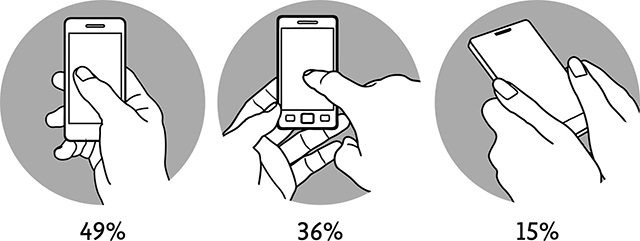
\includegraphics[width=\textwidth]{images/MobileWeb-Fitts}	
						\caption[Mobile Web - Impugnature e utilizzo] {Mobile Web - Tipi di impugnatura e percentuale di utilizzo}
						\label{fig:MobileWeb-Fitts}
					\end{figure}
					
					Come si vede dalla figura ~\ref{fig:MobileWeb-Fitts}, l'uso del pollice è preferito (75\%) e questo garantisce una \textbf{pessima precisione}. Ci sono poi delle zone di \textbf{bassa usabilità} perché raggiungibili solo allungando la mano, nel caso dei tablet peggio ancora, per questo i controlli dovrebbero essere sempre nella parte inferiore (come i controlli standard degli smartphone). Bisogna poi tenere conto che la forma dello schermo può cambiare da normale a landscape. La migliore interfaccia quindi deve tenere conto di tutti i casi e lasciare la possibilità all'utente di cambiare interfaccia.
					\paragraph{Zone magiche}
						Riguardo le così definite \emph{zone magiche} su mobile non disponiamo di nessuna finestra. I \emph{fan menu} funzionano molto bene meno invece i \emph{pie menu} perché le dita coprono parti di schermo e quindi anche pulsanti.
					